\section{The Language}\label{sec:lang}
%
This section presents an overview of the conceptual modeling language.
The \emph{concrete syntax} will be presented using an example in subsection \ref{subsec:example}. 
In subsection \ref{subsec:ast},
the example's model is shown as an \emph{abstract syntax tree} parsed by the CML compiler.
The mapping of the CML example to other modeling notations is illustrated in subsection \ref{subsec:mapping}.
The CML metamodel (the \emph{abstract syntax}'s structure) will be presented in subsection \ref{subsec:metamodel}. 
(The appendix \ref{sec:spec} provides a formal description of the \emph{concrete syntax},
along with its mapping to the \emph{abstract syntax}.) Finally, subsection \ref{subsec:expr} defines the semantics of CML expressions.

\subsection{An Example}\label{subsec:example}

On the example of figure \ref{fig:store}, some concepts, such as \emph{Book} and \emph{Customer}, are declared in CML.
The block-based syntax declaring each concept resembles the C \cite{clang} language's syntax.
Each concept declares a list of properties.
The property declarations are based on the Pascal \cite{pascal} style for variable declarations,
where the name is followed by a colon (``:'') and then the type declaration.
Part of the CML syntax for expressions, such as the expression in \emph{BookStore}'s \emph{orderedBooks}, is based on OCL \cite{ocl} expressions; while the syntax of the expression in \emph{goldCustomers} is new, its semantics also match OCL \cite{ocl} query expressions.

\begin{figure}
\verbatimfont{\small}
\begin{verbatim}
concept BookStore
{
    books: Book+;
    customers: Customer*;
    orders: Order*;
    /goldCustomers = customers | select totalSales > 1000;
    /orderedBooks = orders.items.book;
}

concept Book
{
    title: String;
    price: Decimal;
    quantity: Integer = 0;
}

concept Customer
{
    orders: Order*;
    /totalSales = orders | collect result += total;
}

concept Order
{
    customer: Customer;
    total: Decimal;
}

association CustomerOrder
{
    Order.customer: Customer;
    Customer.orders: Order*;
}
\end{verbatim}
\caption{The example above is adapted to CML from the fictional Livir bookstore, which is presented as a case study in Wazlawick \cite{wazlawick}.}
\label{fig:store}
\end{figure}


The key language features are:
\emph{Book} and \emph{Customer} are concepts;
\emph{title} and \emph{price} under the \emph{Book} concept are attributes;
\emph{totalSales} under the \emph{Customer} concept is a derived attribute;
the \emph{books} and \emph{customers} properties declared under the \emph{BookStore} concept represent unidirectional associations (in UML \cite{uml}, they would correspond to the association roles);
\emph{CustomerOrder} binds two unidirectional associations
(represented by the \emph{orders} property under the \emph{Customer} concept
and by the \emph{customer} property under the \emph{Order} concept)
into a single bidirectional association;
the \emph{goldCustomers} and \emph{orderedBooks} properties under the \emph{BookStore} concept are examples of derived associations. These language features will be defined in the subsection \ref{subsec:metamodel}.

\subsection{The Abstract Syntax Tree}\label{subsec:ast}

The \emph{BookStore} concept\footnote{For brevity,
only displaying the partial tree of the CML model defined in figure \ref{fig:store} (just for the \emph{BookStore} concept), 
but a similar tree is generated by the compiler for all other concepts.}
specified in the model of figure \ref{fig:store},
when parsed and instantiated by the CML compiler,
generates the abstract syntax tree (or AST for short) in figure \ref{fig:ast}.

\begin{figure}
\centering
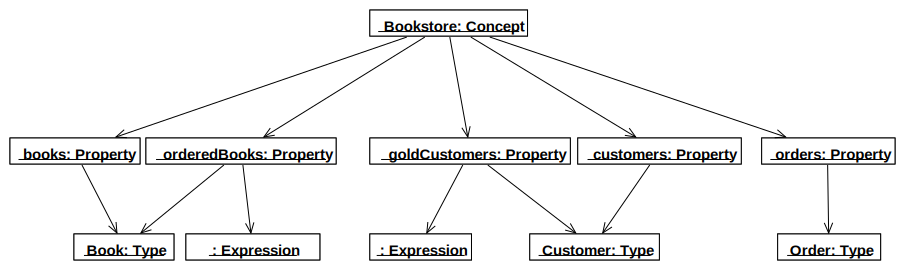
\includegraphics[width=\textwidth]{language/figure-ast}
\caption{The abstract syntax tree generated by the CML compiler after parsing the \emph{BookStore} concept.
TODO: Add "set" nodes to the AST.}
\label{fig:ast}
\end{figure}

The resultant AST in figure \ref{fig:ast} is the CML compiler's internal representation of the \emph{BookStore} concept,
as specified by the model in the CML source listed in figure \ref{fig:store}. 
Using EMOF's terminology \cite{mof},
each node in figure \ref{fig:ast} represents an instance of a class from the CML metamodel.
The root-level node is an instance of the \emph{Concept} class. 
Its subnodes are instances of the \emph{Property} class,
which in turn have (as subnodes) instances of the \emph{Type} and \emph{Expression} classes.

Once generated internally by the CML compiler,
the AST in figure \ref{fig:ast} will be used as the input for the extensible templates during the code generation phase,
shown in section \ref{sec:compiler}.

In order for the CML compiler to successfully generate the AST,
it is necessary to define the CML metamodel,
which is presented in subsection \ref{subsec:metamodel}.
Before, subsection \ref{subsec:mapping} explores the mapping of conceptual models defined with CML to other modeling notations.


\subsection{Mapping CML Source to UML and OCL}\label{subsec:mapping}

Part of the CML metamodel (presented in section \ref{subsec:metamodel})
may be considered a small subset of the UML  \cite{uml} metamodel.
Thus, the structural (static) elements of CML models can be transformed into UML class diagrams.
The example CML model in the listing of figure \ref{fig:store} is mapped to the UML model in figure \ref{fig:uml}.

\begin{figure}
\centering
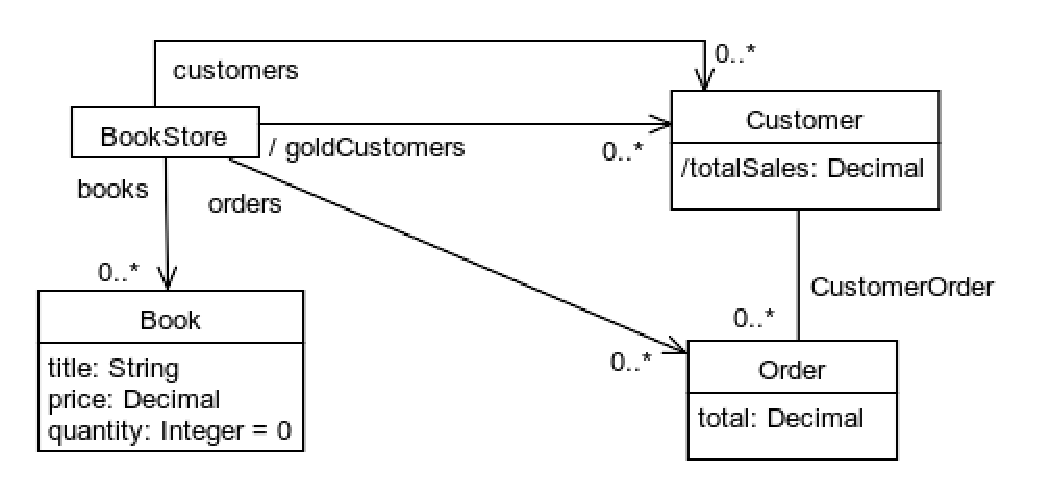
\includegraphics[width=0.8\textwidth]{language/diagram-uml}
\caption{The UML class diagram \cite{uml} for the CML model listed in figure \ref{fig:store}.}
\label{fig:uml}
\end{figure}

In figure \ref{fig:uml},
the CML concepts (\emph{BookStore}, \emph{Book}, \emph{Customer} and \emph{Order})
are mapped to corresponding UML classes.
The CML properties that represent attributes
(such as \emph{title}, \emph{quantity} and \emph{price} of \emph{Book})
are mapped to UML attributes under each class.
The CML properties that represent unidirectional associations
(\emph{books}, \emph{customers}, and \emph{goldCustomers} of \emph{BookStore})
are mapped to UML associations with corresponding roles
(showing the navigability direction, and matching the property names and cardinality.)
The CML bidirectional association \emph{CustomerOrder}
(comprised by two CML properties: \emph{Customer.orders} and \emph{Order.customer})
is mapped to a UML association with bidirectional navigability (that is, no direction arrow.)
As demonstrated by this example,
CML strives to enable modeling at the same conceptual level as allowed by UML.
That being said, when compared to the UML metamodel,
the CML metamodel supports only a core set of its elements,
as shown in subsection \ref{subsec:metamodel}.

Besides the structural elements of a conceptual model (as seen above),
CML also has expressions that can set initial values to attributes,
and define derived properties for both attributes and associations.
CML expressions are partially based on the OCL \cite{ocl} syntax,
but they follow closely the OCL semantics.
For example,
the following CML expression (extracted from figure \ref{fig:store}) is
a path-based navigation expression borrowed from OCL:

\verbatimfont{\small}
\begin{verbatim}
/orderedBooks = orders.items.book;
\end{verbatim}

Using association properties,
the expression above navigates from one instance of \emph{BookStore},
passing through all linked \emph{orders},
and then through all \emph{items} of all \emph{orders},
in order to return all books that have been ordered.
As another example, the following CML expression
(also extracted from figure \ref{fig:store}) does not follow the OCL syntax:

\verbatimfont{\small}
\begin{verbatim}
/goldCustomers = customers | select: totalSales > 1000;
\end{verbatim}

However, the expression above closely matches the semantics of the following OCL expression:

\verbatimfont{\small}
\begin{verbatim}
derive: customers->select(totalSales > 1000)
\end{verbatim}

Both the CML expression and the OCL excerpt above evaluate to a set of \emph{Customer} instances
that have bought more than 1000 in the \emph{BookStore}.

The OCL syntax for expressions that process collections of instances has the following general form:

\verbatimfont{\small}
\begin{verbatim}
collection->method_name(predicate or function)
\end{verbatim}

The expression above is based on method invocations
(an influence from UML's object-oriented paradigm),
and thus it has an imperative style.
CML, on the other hand, intends to be agnostic towards programming paradigms.
By using extensible comprehensions \cite{trinder}
to define derived attributes and associations,
CML's syntax is more declarative,
similar to SQL \cite{sql} or C\#'s LINQ \cite{torgersen}.
In CML, smaller expressions can also be combined into larger ones. For example:

\verbatimfont{\small}
\begin{verbatim}
/goldOrders = for order in bookStore.orders,
                  goldCustomer in bookStore.goldCustomers
                  | select: order.customer == goldCustomer | yield: order
 \end{verbatim}

Above, all \emph{orders} from \emph{goldCustomers} are returned.
The sub-expressions are evaluated sequentially:
the \emph{for} expression provides a cross join of all (\emph{order}, \emph{goldCustomer}) pairs;
the \emph{select} expression selects only the pairs that have matching customers;
Finally, the \emph{yield} expression maps selected pairs into a sequence of \emph{orders}.
Sub-expressions like \emph{for}, \emph{select} and \emph{yield} can be combined in different configurations
in order to derive any required attributes and associations.

\subsection{The CML Metamodel (Abstract Syntax)}\label{subsec:metamodel}

In the article \emph{UML and OCL in Conceptual Modeling}, 
Gogolla \cite{gogolla} shows, by mapping the UML \cite{uml} metamodel to the ER \cite{er} metamodel,
how UML models (augmented by OCL \cite{ocl} constraints) can be used to specify conceptual models.
Also, Wazlawick \cite{wazlawick} systematically prescribes in his book a method for conceptual modeling using UML and OCL. 

Since one key CML goal is enabling the specification of conceptual models
(such as those specified by ER models and UML/OCL models),
in order to present the key elements of the CML metamodel,
a similar approach to Gogolla's is used to map the CML metamodel to the ER metamodel,
and to the UML/OCL metamodel.

\pagebreak[4]

The EMOF \cite{mof} model presented by figure \ref{fig:metamodel} is a simplified version of the CML metamodel:

\begin{figure}
\centering
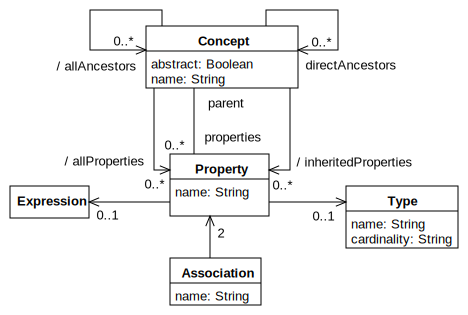
\includegraphics[width=0.8\textwidth]{language/diagram-metamodel}
\caption{This class diagram renders the EMOF \cite{mof} model defining the CML metamodel.}
\label{fig:metamodel}
\end{figure}

In CML metamodel shown in figure \ref{fig:metamodel},
a \emph{Concept} is composed of zero-or-more \emph{Property} instances.
Each \emph{Property} may have a \emph{Type} and an \emph{Expression}.
If two \emph{Property} instances represent the same bidirectional association,
there must be an \emph{Association} instance that binds them.
Unidirectional associations are only represented by the \emph{Property} instance (representing the association role)
that enables the navigation from the source \emph{Concept} instance to the target one (which is represented by the property's \emph{Type}.)

Next, there is a description for the key metamodel elements.

\subsubsection{Concept.}

According to Wazlawick \cite{wazlawick},
a concept represents complex information that has a coherent meaning in the domain.
They aggregate attributes and cannot be described as primitive values.
They may also be associated with other concepts.
On the ER metamodel, it is known as \emph{entity};
on the UML metamodel, as \emph{class}.

\subsubsection{Property.}

May be an attribute holding values of primitive types,
or references (or collections of references) linking concepts.
On the ER metamodel,
the set of all references is known as \emph{relationship};
on the UML metamodel, unidirectional associations.
Attributes have the same name on all metamodels.

\subsubsection{Association.}

Unlike the ER and UML metamodels, in the CML metamodel, only bidirectional associations are represented with the Association class. They bind the non-primitive properties (from the same or from different concepts.) 


\subsubsection{Type.} They may be primitive types (such as Boolean, String, Decimal, and Regex), references to concept instances, or still collections of concepts. They may also be optional, meaning their value may or may not have been set.

\subsection{CML Expressions}\label{subsec:expr}


